\section{Optimization}

If the closed form is not available or desirable, as calculating it is expensive, we use the \textbf{gradient descent} algorithm. It works by initializing $w^0$ and iteratively moving it towards the optimal solution. We choose the direction by calculating $\nabla \ell(w)$ and then multiply it by the stepsize / learning rate $\eta$:
$$w^{t+1} = w^t - \eta_t \cdot \nabla \ell(w^t)$$

Convergence is only guaranteed for the convex case, else we might get stuck at any stationary point. 

\begin{center}
	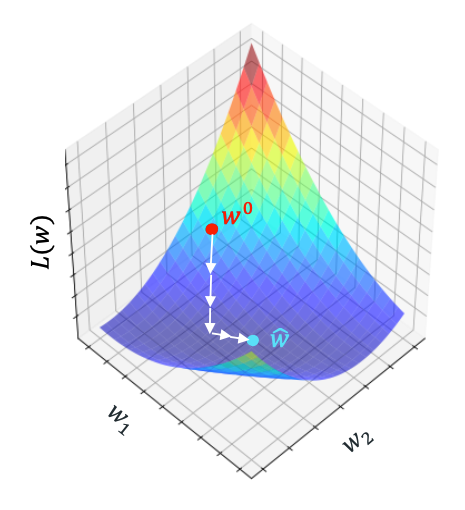
\includegraphics[width=0.6\columnwidth]{gradient-descent.png}
\end{center}

As the slope gets smaller, we want to decrease $\eta$, so that we do not overshoot. For the linear regression case we have:
$$||w^t - w^*||_2 \leq \rho^t ||w^0 - w^*||_2, \quad \rho = ||I - \eta X^\top X||_{op}$$

Where $\rho$ is the convergence speed for constant stepsize $\eta$. This leads to an optimal fixed stepsize of:
$$\eta = \frac{2}{\lambda_{\text{min}} + \lambda_{\text{max}}}$$

We stop when new iterations does not change anymore (below a certain threshold).

To make gradient descent more stable / robust against ill-conditioned landscapes we might add momentum:
$$w^{t+1} = w^t + \gamma \Delta w^{t-1} - \eta_t \nabla \ell(w^t)$$

\subsection{Stochastic Gradient Descent}

When we have a lot of data, it is costly to compute the gradient, so we only use a minibatch $S$ of the dataset $D$ (randomly sampled without replacement). Now the update step looks like this:
$$w^{t+1} = w^t - \eta_t \cdot \nabla \ell_S(w^t)$$

Where the loss is only calculated over the minibatch $S$. This method also gives us a chance to escape saddle points.